\documentclass[a4paper]{article}

\usepackage[english]{babel}
\usepackage[utf8]{inputenc}
\usepackage{amsmath}
\usepackage{graphicx}
\usepackage[colorinlistoftodos]{todonotes}

\title{Fine Structure of $H$-Line}

\author{Rakesh Kumar Tiwari}

\date{\today}

\begin{document}
\maketitle

\begin{abstract}
H is simplest atom. Its spectrum was observed by Balmer (1885) in certain type of stars. The theoretical explanation of H- series was explained by Bohr. Sommerfield (1916) introduced the concept of elliptical orbits and special theory of relativity. He proposed that $H_{\alpha}$ and  $H_{\beta}$ consist two strong components and three weaker ones. Further advancement in the theory was with the introduction of spinning electron and spin-orbit interaction (quantum-relativity correction), first done by Heisenberg and Jordon (1926). To some extant, this model was successful to explain many characteristic of fine structure of lines, except discrepancy in the separation between the main component of $H_{\alpha}$ lines. However, the best explanation of experimental observation was proved by assuming $2^{2}P_{\frac{3}{2}}$ is lower than $2^{2}S_{\frac{3}{2}}$, later known as "Lamb Shift". 
\end{abstract}

\section{Introduction}
\label{sec:introduction}

                   
Even the hydrogen spectrum, the simplest of all systems, is observed to have a fine structure. Michelson studied the Balmer lines with interferometer and found that both H and H were doublets with separations of only 0.14 and 0.08 Å, or 0.32 and 0.33 cm-1, respectively
                   
The most informing observations that have been made on hydrogen like atoms are those of Paschen  on the singly ionized helium line  of wavelength 4686 Å. This line  corresponds to the first member of the so-called Paschen series of hydrogen

\section{Sommerfield Relativity Correction}
\label{sec:theory}

\subsection{Extension of Two-dimensional to Three-dimensional elliptical orbit }
The extension of Bohr's atomic by Sommerfeld to include elliptic orbits adds no new energy levels to the hydrogen atom. For a given total quantum number n, all elliptic orbits s, p, d, . . . have just the same energy as the Bohr circular orbits with the same n. This energy in wave number is 
\begin{equation}
    \frac{E_n}{hc}=-\frac{RZ^2}{n^2}=-T
\end{equation}
Where R is Rydberg Constant, and h is Planck's constant.



\subsection{Sommerfied 's relativistic correction }
Bohr pointed out in his earliest papers that the relativistic change of the orbital electron should be taken into account in computing the energy levels. Introducing elliptic orbits, Sommerfeld applied the special theory of relativity to the electron levels. Due to the different velocity of the electron in orbits of the same but differing azimuthal quantum number, the mass of the electron and hence the resultant energy levels are all different. If the rest mass of the electron is $m_a$, its mass when moving with velocity v is given by the special theory of relativity as
By the special theory of relativity $m = m_0 (1 -\frac{v^2}{c^2} )^\frac{1}{2}$

Where m is the mass of  electron, c is speed of light.If M is of the mass of nucleus $$\mu=\frac {mM}{m+M}$$
As result of this change in mass, the relativity change in mass, which is greatest at perihelion and  greatest for the most elliptic orbits, there is an advance of the perihelion, or precession of the electron orbit, similar  to that of the planet Mercury moving about the sun. This precession is shown schematically in Fig. 9.2.

\begin{figure}
\centering
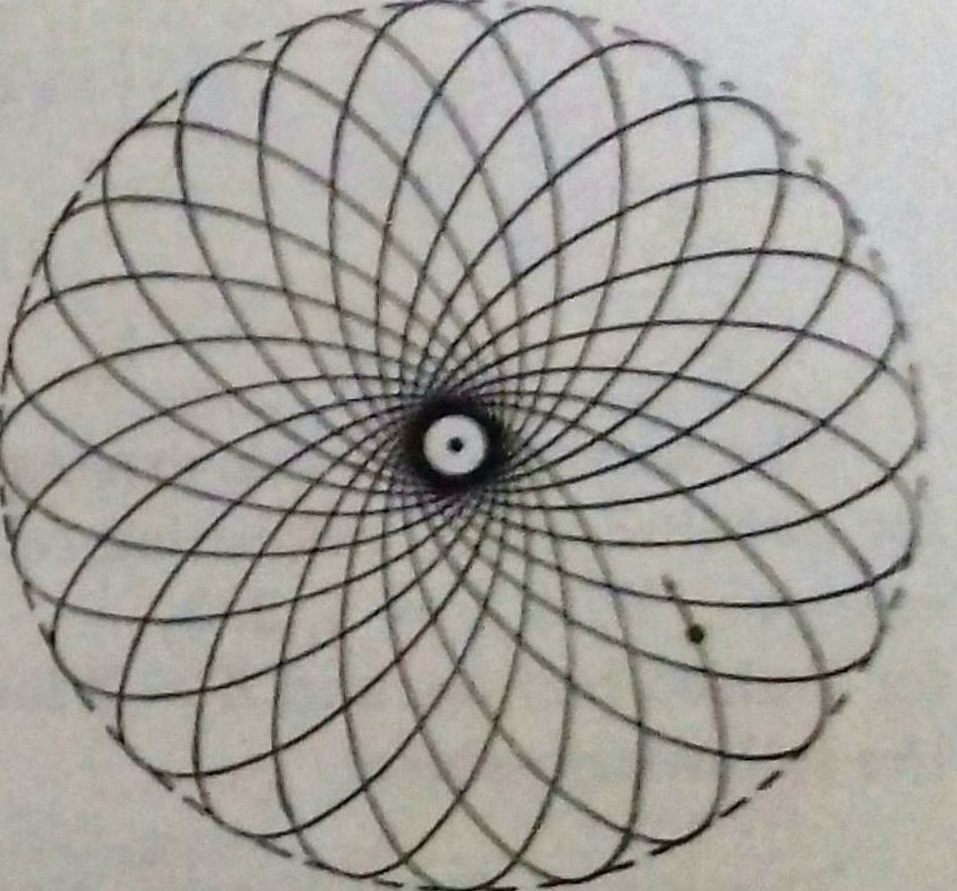
\includegraphics[width=0.3\textwidth]{Relativistic_orbit.jpg}
\caption{\label{fig:frog} Schematic representation of precession of an electron in atomic orbital.}
\end{figure}

The energy of such type of energy levels in wave number is given by 

\begin{equation}
\begin{split}
T & = - \frac { W } { h c }   \\
  & = \frac { R Z ^ { 2 } } { n ^ { 2 } } \\
  &\quad + \frac { R \alpha ^ { 2 } Z ^ { 4 } } { n ^ { 4 } } \left[ \frac { n } { k } - \frac { 3 } { 4 } \right] + \frac { R \alpha ^ { 4 } Z ^ { 6 } } { n ^ { 6 } }\left[ \frac { 1 } { 4 } \left( \frac { n } { k } \right) ^ { 3 }  + \frac { 3 } { 4 } \left( \frac { n } { k } \right) ^ { 2 } - \frac { 3 } { 2 } \left( \frac { n } { k } \right) + \frac { 5 } { 8 } \right] \\
  \quad + .....
\label{eq:sn}
\end{split}
\end{equation}

The first term of this expansion is the same as that derived by Bohr for circular orbits, neglecting relativity, and gives the major part of the energy. With n = 1, 2, 3, , and with Z = 1 for hydrogen, Z = 2 for ionized helium, and Z = 3 for doubly ionized lithium.
                   
To each of these values corrections from Eq. (9.6) must be added. For small values of Z the first term involving $Z^4$ and $\alpha^2$ is the only one of importance and the third and succeeding terms may be neglected.

Therefore, corrections to be added to each of the term values found by Bohr's orbital theory is following
\begin{equation}
    \delta T = \frac{ R \alpha ^ { 2 } Z ^ { 4} } { n ^ { 4 } }\left[ \frac { 1 } { 4 } \left( \frac { n } { k } \right) ^ { 3 }  + \frac { 3 } { 4 }\right]
\end{equation}


Observed Hydrogen Fine diagrams of the theoretical fine structure of the first two lines of the Balmer series of hydrogen are shown in Fig. 9.4. Applying selection and intensity rules, both $H_\alpha$ and $H_\beta$ should be composed of two strong components and three weaker ones. Until 1947, neither one of these patterns had ever been resolved into more than two components. Later, these lines were further resolved in a microwave experiment performed by Lamb and Ratherford in 1947, contradicted the both Sommerfield and Dirac's theory.
\begin{figure}
    \centering
    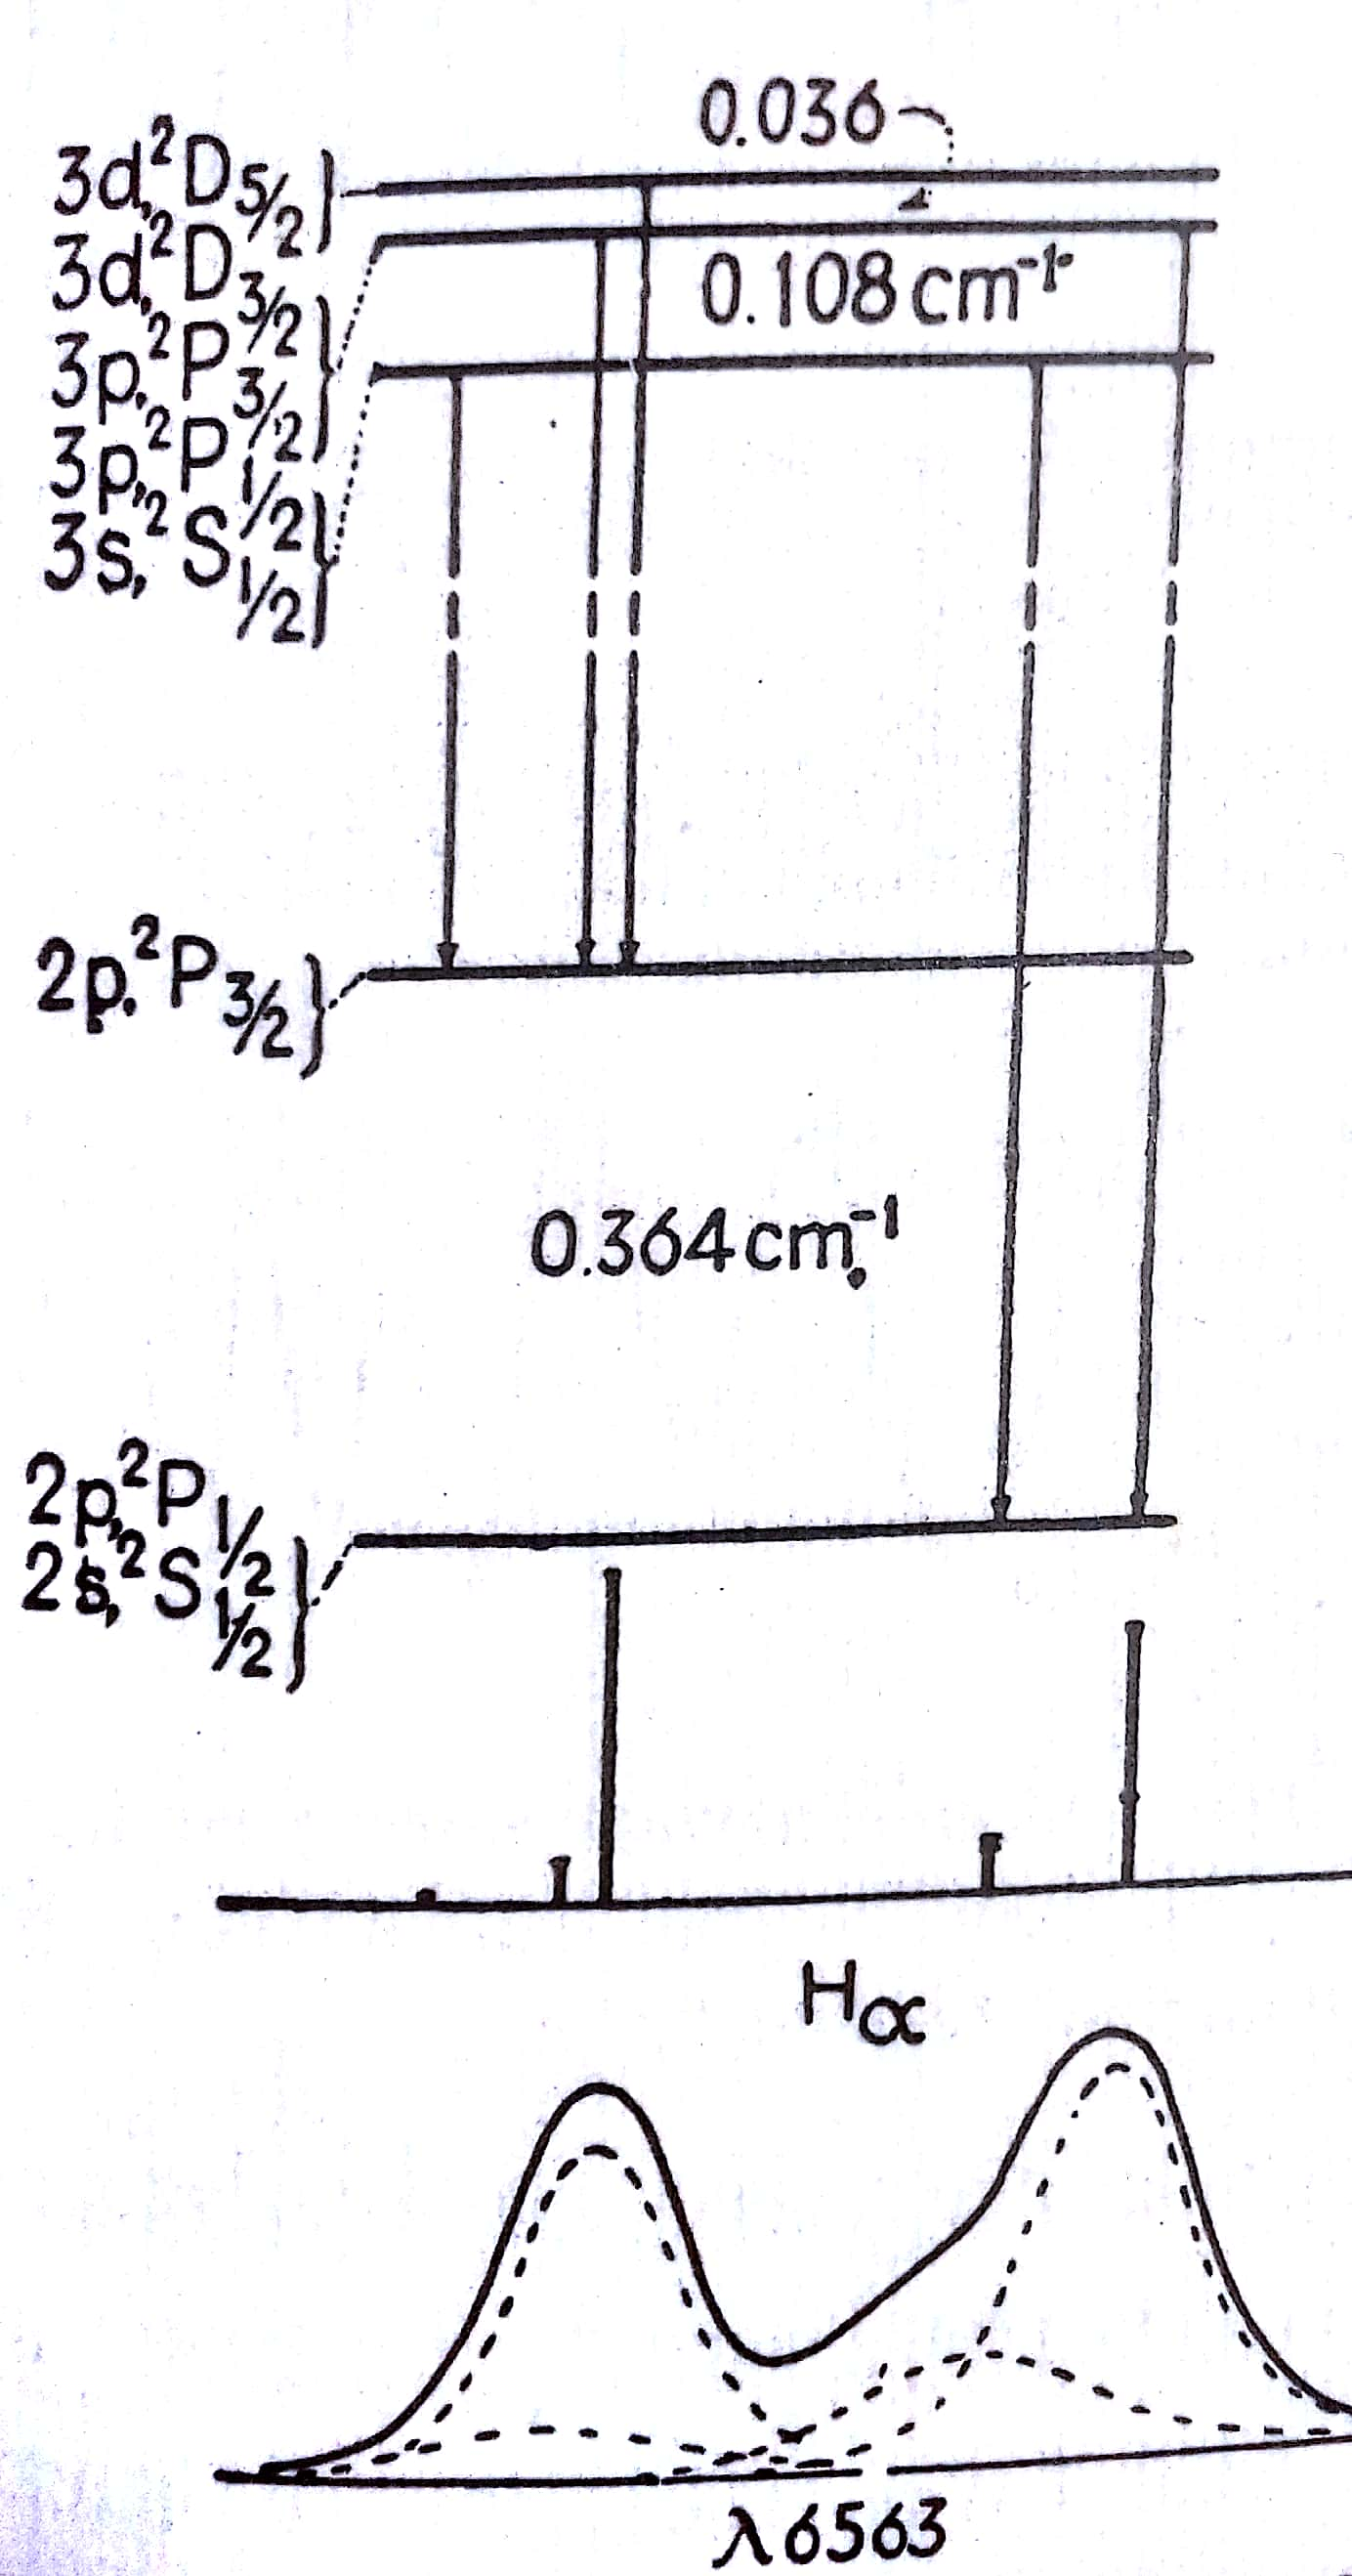
\includegraphics[width=.4\textwidth]{fineH.jpg}
    \caption{Caption}
    \label{fig:my_label}
\end{figure}
\section{Lamb's Shift}

For H atom, a particular $n$ value with same $j$ value but different $l$ values, such as $2^2P_\frac{1}{2}$ and $2^2S_\frac{1}{2}$ are not degenerate, but are separated.\\
\begin{figure}
    \centering
    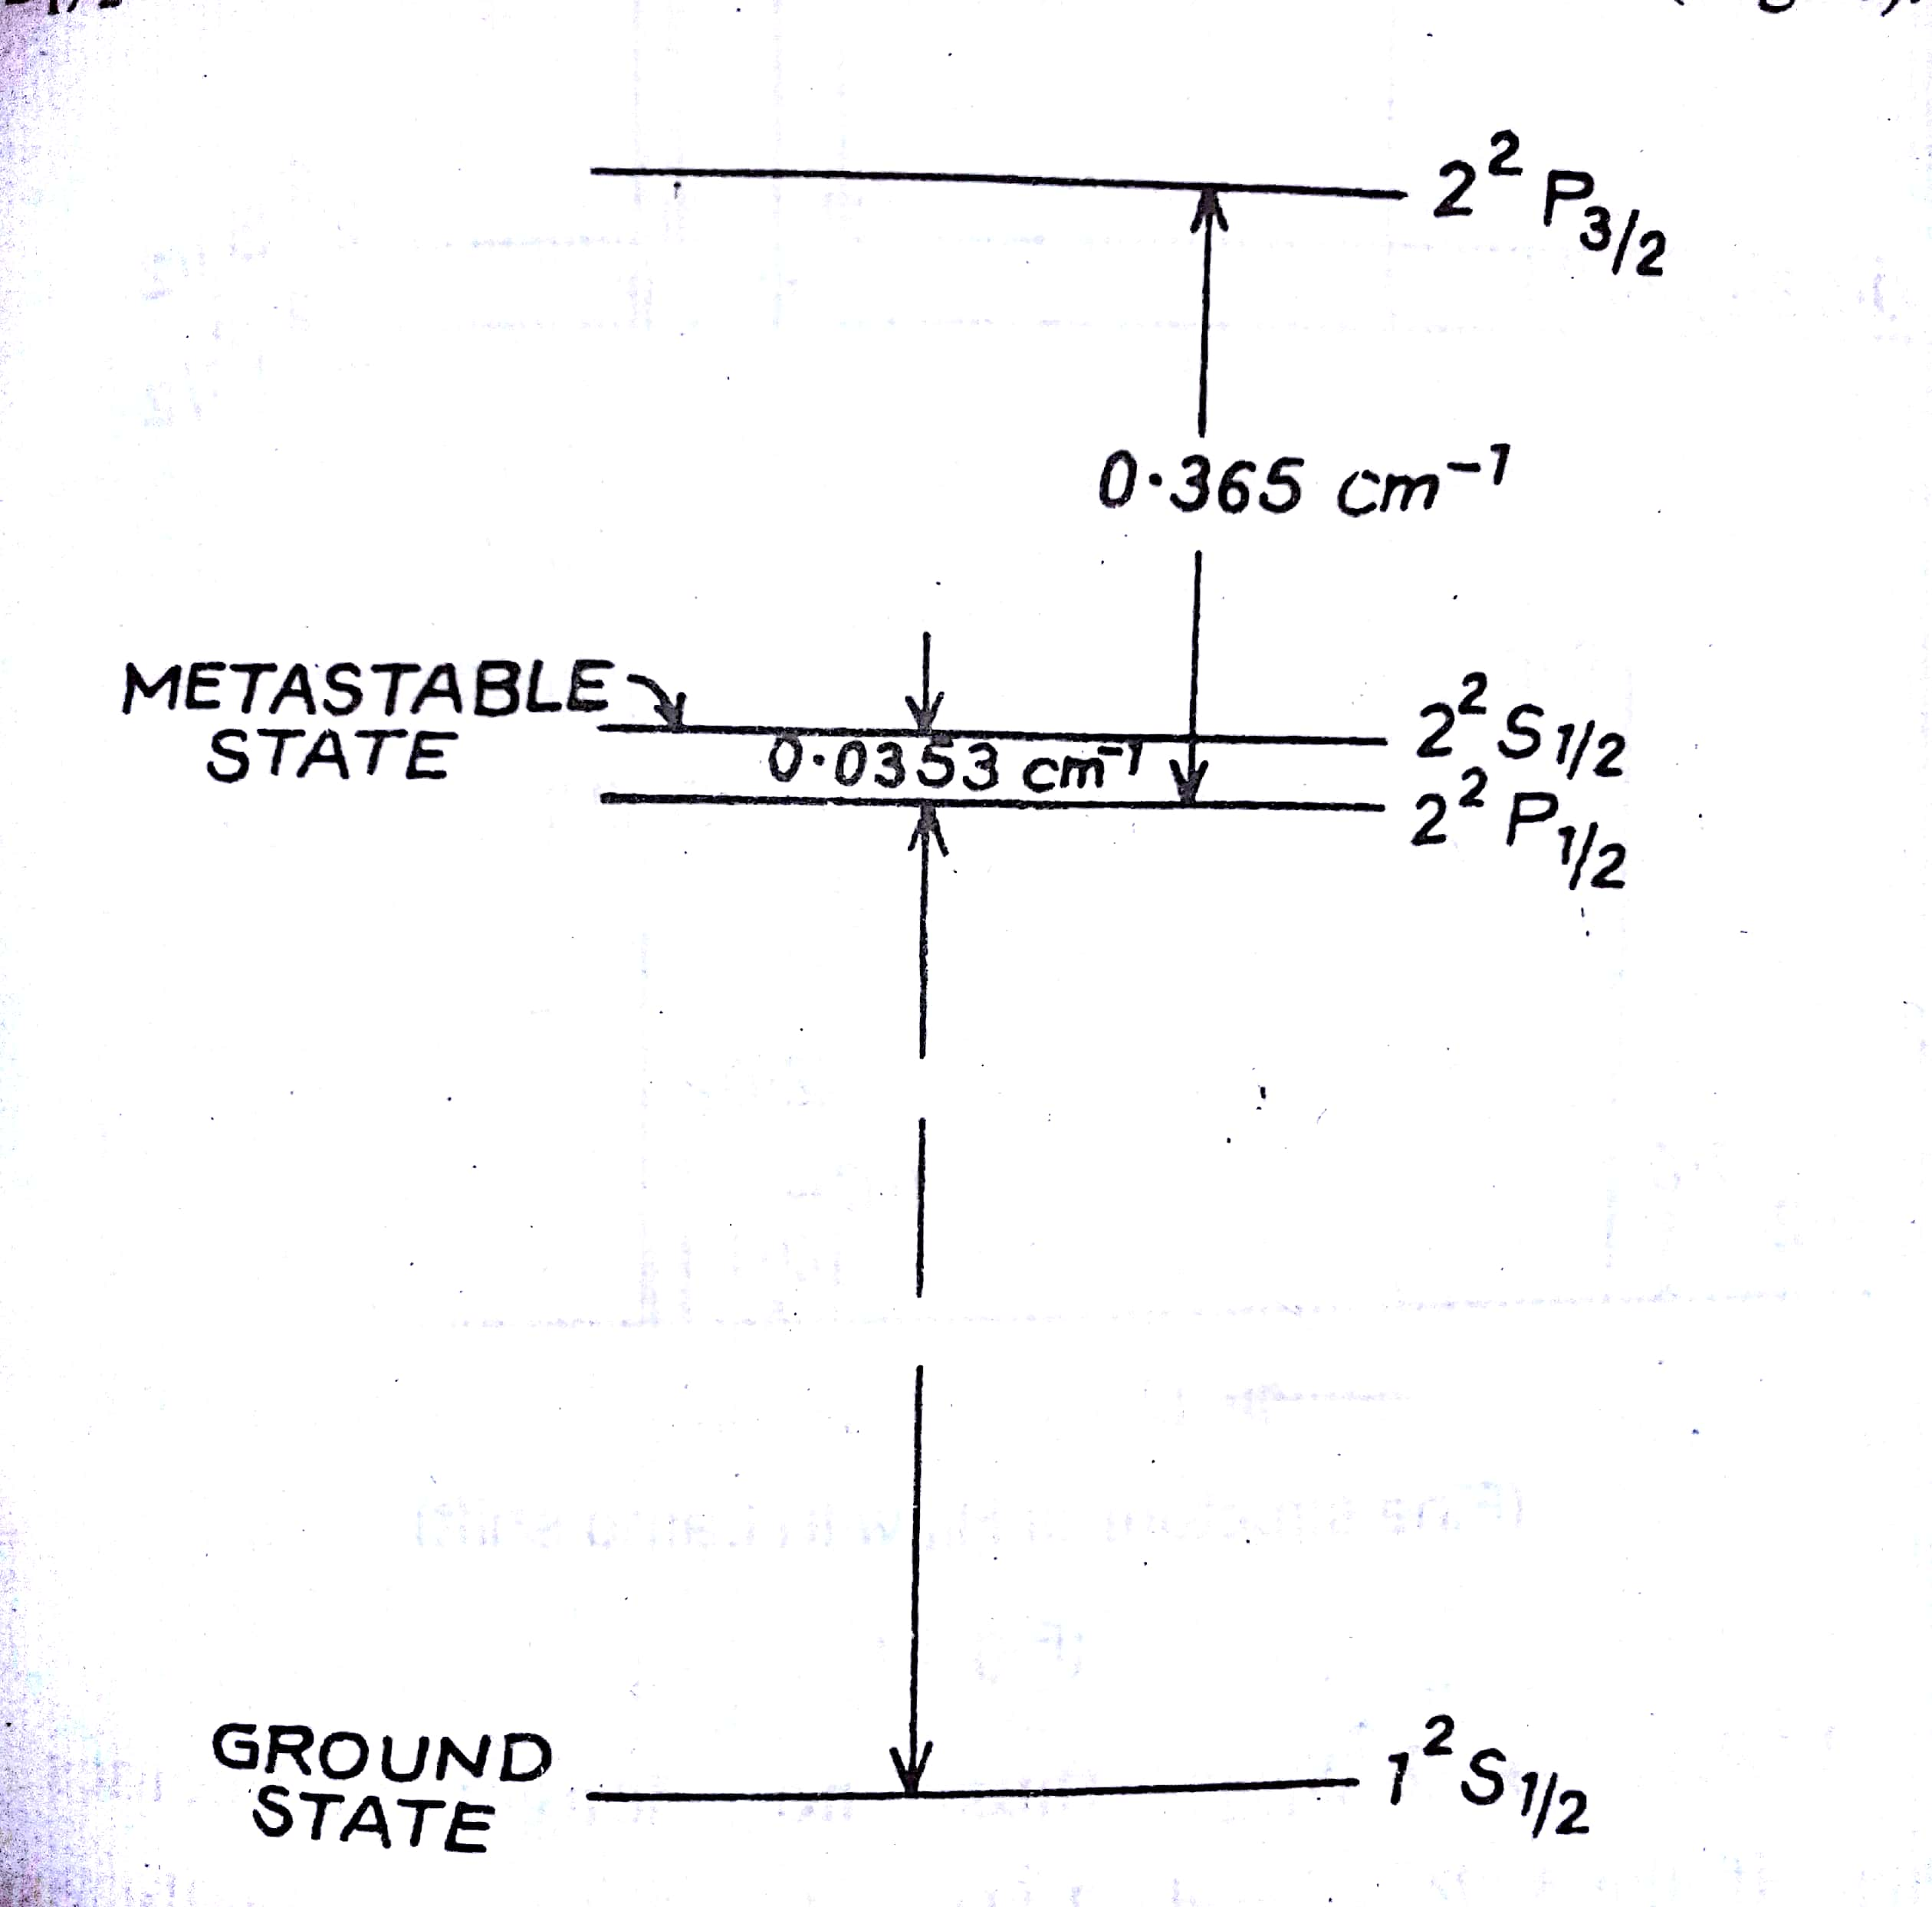
\includegraphics[width=.4\textwidth]{lamb2.jpg}
    \caption{Lamb Shift}
    \label{fig:fig2}
\end{figure}
For example in fine structure of $H_\alpha$,  $2^2P_\frac{1}{2}$ is lower than 0.035 $cm^{-1}$  $2^2S_\frac{1}{2}$ energy level. Thus fine structure of $H_\alpha$ consists 7(seven)s
line shown in figure .

\begin{figure}
    \centering
    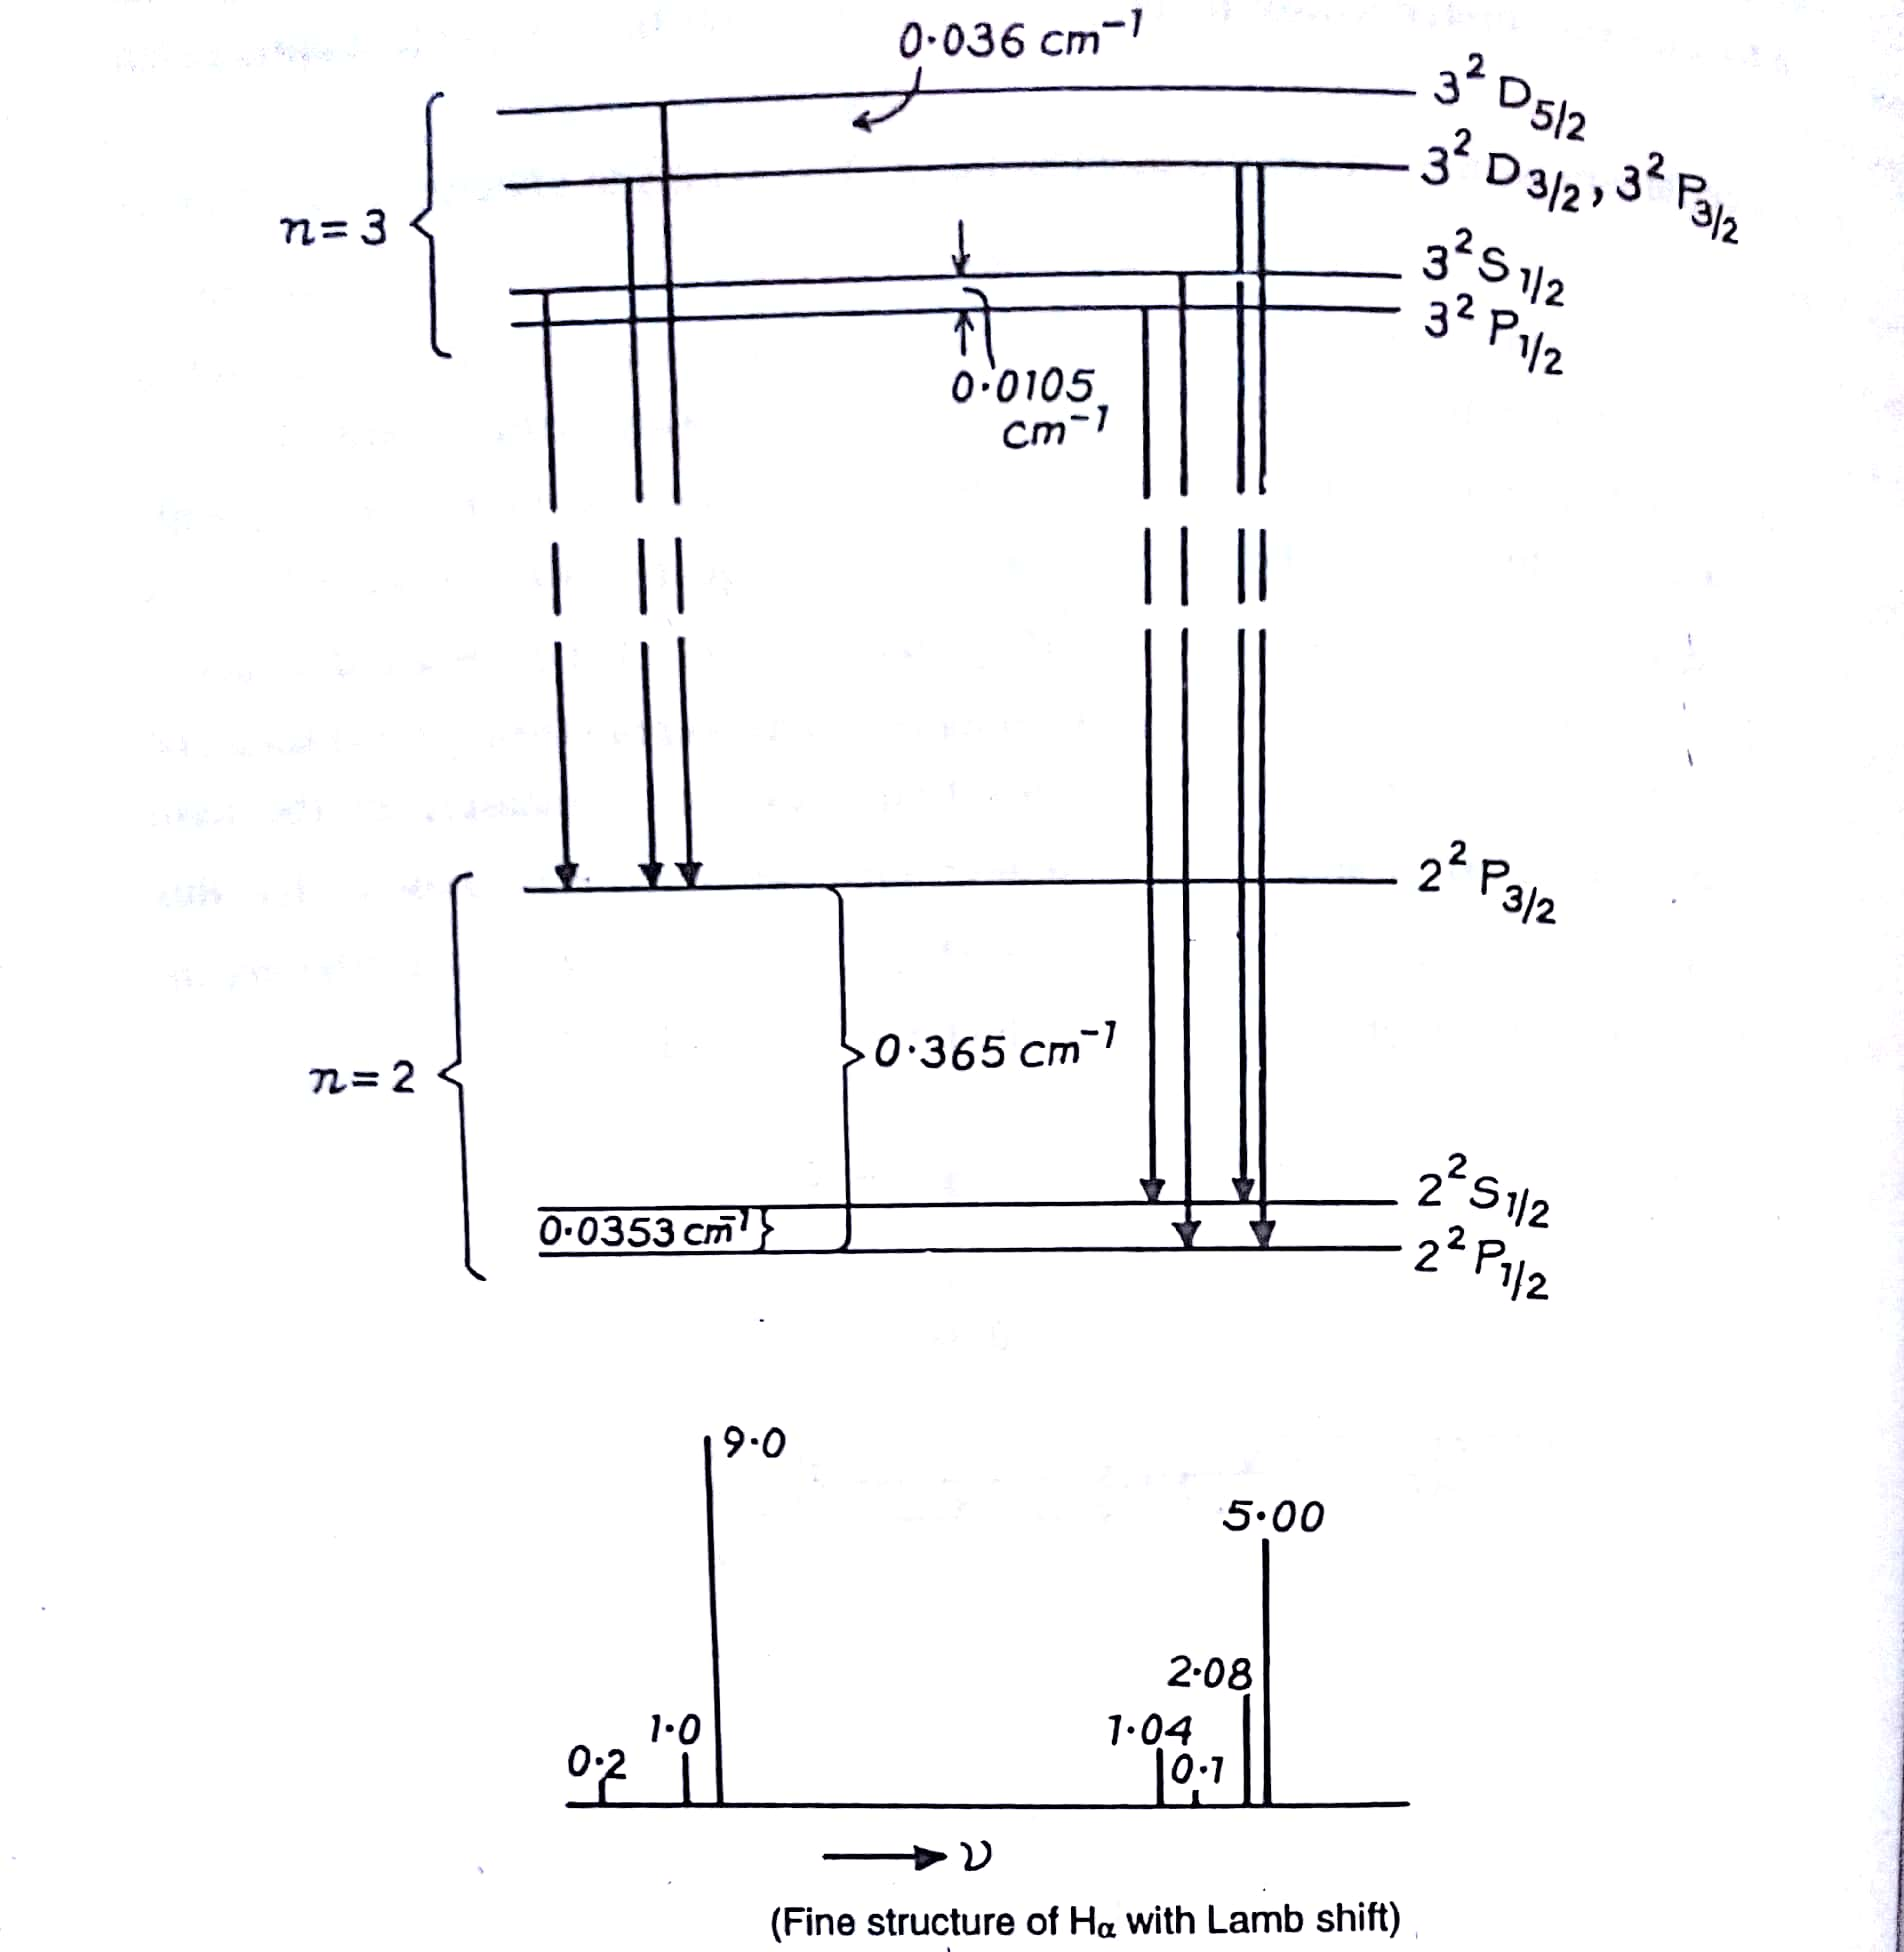
\includegraphics[width=.5\textwidth]{lamb3.jpg}
    \caption{Fine structure of Lamb shift in H atom}
    \label{fig:fig3}
\end{figure}












\begin{thebibliography}{9}
\bibitem{nano3}
  H., White
  \emph{Atomic Spectra}.
 McGRAW HILL publication

\end{thebibliography}
\begin{thebibliography}{9}
\bibitem{nano4}
  A. Bea
  \emph{Atomic Spectra}.
 McGRAW HILL publication

\end{thebibliography}\end{document}